\documentclass[12pt,letterpaper]{article}

\usepackage{amsmath}
\usepackage{fancyhdr}
\usepackage{graphicx}
\usepackage{verbatim}
\usepackage{minted}

\usepackage{mathtools}
\DeclarePairedDelimiter\abs{\lvert}{\rvert}
\makeatletter
\let\oldabs\abs
\def\abs{\@ifstar{\oldabs}{\oldabs*}}
\makeatother

\pagestyle{fancy}
\lhead{Marco Muzio}
\rhead{Homework \#1 - Computational Physics}

\begin{document}

\subsection*{1.}

The code written to implement each of the algorithms can be found in the source code \verb|prob1.cpp| in the appendix. Figures 1-3 below show the log-log plots of the relative error $\epsilon_r$ of each method as a function of the step size $h$. Plots and their data were generated by running \verb|prob1.sh|, which can also be found in the appendix.

\begin{figure}[H]
	\centering
	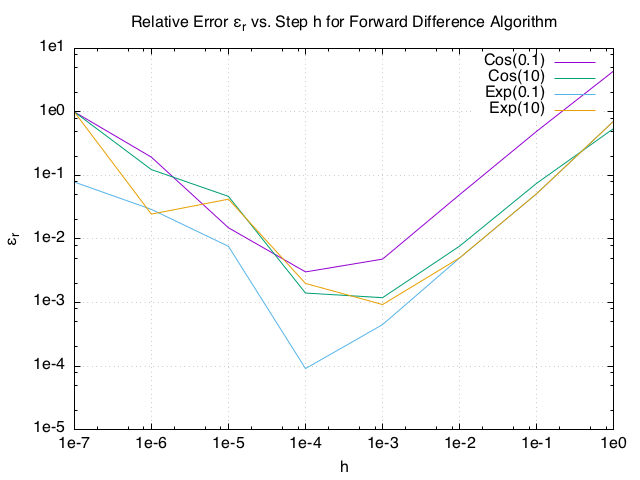
\includegraphics[scale=0.6]{forward_diff.png}
	\caption{Relative error of the derivative of $\cos(x)$ and $\exp(x)$ for $x=0.1,10$ calculated using the forward differences algorithm as a function of the step $h$.}
\end{figure}

We have the following estimates for the optimal step $h_{opt}$ and optimal relative error $\epsilon_r$ for a forward difference algorithm from class:

\begin{equation}
	h_{opt} \sim \sqrt{\abs{\frac{f(x_o)}{f''(x_o)}} \epsilon_m}
\end{equation}
\begin{equation}
	\epsilon_{opt} \sim \sqrt{\epsilon_m}
\end{equation}

where $x_o$ is the point for which the derivative is being calculated, $\epsilon_m$ is the machine precision which we take to be $\sim 10^{-7}$, and $f$ is the function whose derivative is being calculated. (2) corresponds to an optimal error of $\epsilon_{opt} \sim 10^{-4}$. Looking at Figure 1, we see the minimum relative errors range from $10^{-3}-10^{-4}$, in good agreement with out rough estimate for $\epsilon_{opt}$. The table below lists the estimated value of the optimal step $h_{opt}$ as given by (1).

\begin{table}[h]
	\centering
	\begin{tabular}[h]{| c | c |}
		\hline
		$f(x_{o})$	&	$h_{opt}$ \\ \hline \hline
		$\cos(0.1)$	&	$\sim 10^{-4}$	\\ \hline
		$\cos(10)$ &	$\sim 10^{-4}$	\\ \hline
		$\exp(0.1)$	& 	$\sim 10^{-4}$	\\ \hline
		$\exp(10)$	&	$\sim 10^{-4}$	\\ \hline
	\end{tabular}
\end{table}
	
Comparing the values in the table to the position of the minimum relative error in Figure 1 ($h=10^{-3}-10^{-4}$ for all), we see that the table and the plots are in good agreement. For a forward difference algorithm we expect the truncation error $\epsilon_{T}$ and round-off error $\epsilon_{RO}$ to be estimated by the following:
\begin{equation}
	\epsilon_{RO} \propto \frac{1}{h}
\end{equation}
\begin{equation}
	\epsilon_{T} \propto h
\end{equation}
Looking at the region of the plots in Figure 1 for $h>h_{opt}$ the $\epsilon_{r}(h)$ are straight lines in the log-log plot, indicating that $\epsilon_{r} \sim h^{n}$ for some positive integer $n$. It is clear from the plot that the $\epsilon_{r}$ increases by a factor of $10$ when $h$ increases by a factor of $10$, indicating the slope of the line in the log-log plot is roughly $1$. Thus, $n\approx 1$ as expected.\\\\

Looking at the region of the plots in Figure 1 for $h<h_{opt}$ the $\epsilon_{r}(h)$ look to be roughly following straight lines. This time the log-log slope of most of these lines looks to be approximately $-1$, indicating that $n\approx-1$ as we expect.\\ 

\begin{figure}[H]
	\centering
	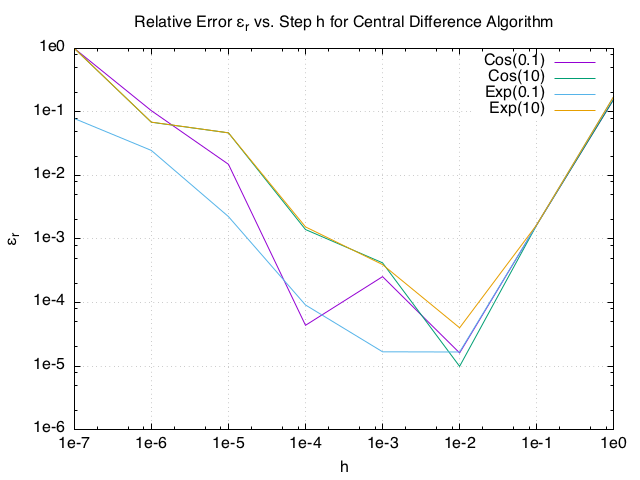
\includegraphics[scale=0.6]{central_diff.png}
	\caption{Relative error of the derivative of $\cos(x)$ and $\exp(x)$ for $x=0.1,10$ calculated using the central differences algorithm as a function of the step $h$.}
\end{figure}

For a central difference algorithm we have the following estimates for $h_{opt}$ and $\epsilon_{opt}$ from class:

\begin{equation}
	h_{opt} \sim \left( \abs{\frac{f(x_o)}{f'''(x_o)}} \epsilon_m \right)^{1/3}
\end{equation}
\begin{equation}
	\epsilon_{opt} \sim \epsilon_{m}^{2/3}
\end{equation}

For single-precision measurements, (6) corresponds to an optimal error of $\epsilon_r \sim 10^{-5}$. Looking at Figure 2, we see the minimum relative errors are roughly $10^{-5}$, as expected. The table below lists the estimated value of the optimal step $h_{opt}$ as given by (5).

\begin{table}[h]
	\centering
	\begin{tabular}{| c | c |}
		\hline
		$f(x_o)$	&	$h_{opt}$ \\ \hline \hline
		$\cos(0.1)$	&	$\sim 10^{-3}$ \\ \hline
		$\cos(10)$	&	$\sim 10^{-3}$ \\ \hline
		$\exp(0.1)$	&	$\sim 10^{-4}$ \\ \hline
		$\exp(10)$	&	$\sim 10^{-4}$ \\ \hline
	\end{tabular}
\end{table}

Comparing the values in the table to the position of the minimum relative error for each plot in Figure 2 ($h=10^{-3} - 10^{-4}$ for all) we see that the table and the plots are again in good agreement. For a central difference algorithm we expect the round-off error $\epsilon_{RO}$ to scale as in (3), but we expect the truncation error $\epsilon_{T}$ to this time scale as:
\begin{equation}
	\epsilon_{T} \propto h^{2}
\end{equation}

Looking at the region of the plots in Figure 2 for $h>h_{opt}$, the $\epsilon_{r}(h)$ look to be roughly straight lines in the log-log plot. This time, though, it is clear that the slope of these lines in the log-log plot is roughly $2$, indicating $n\approx2$ as we would expect. \\

Looking at the region of the plots in Figure 2 for $h<h_{opt}$, the $\epsilon_{r}(h)$ look to roughly be following straight lines. For very small $h$, it is clear that these lines have slope of about $-1$ in the log-log plot, indicating $n\approx-1$ as we expect.\\

\begin{figure}[H]
	\centering
	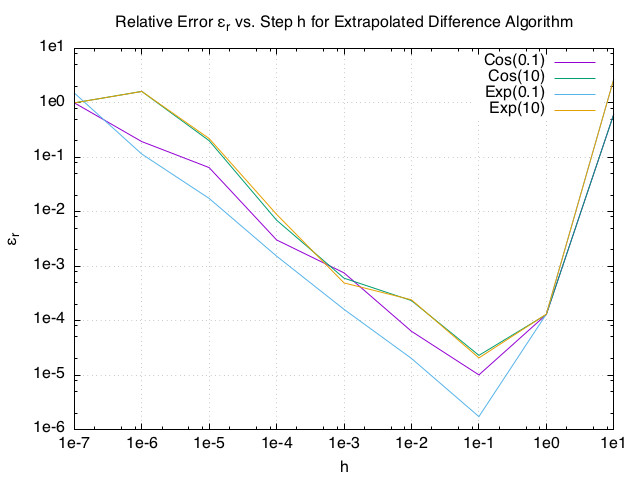
\includegraphics[scale=0.6]{extrap_diff.png}
	\caption{Relative error of the derivative of $\cos(x)$ and $\exp(x)$ for $x=0.1,10$ calculated using the extrapolated differences algorithm as a function of the step $h$.}
\end{figure}

For an extrapolated difference algorithm we have the following estimates for $h_{opt}$ and $\epsilon_{opt}$ from class:

\begin{equation}
	h_{opt} \sim \left( \abs{\frac{f(x_o)}{f^{(5)}(x_o)}} \epsilon_m \right)^{1/5}
\end{equation}
\begin{equation}
	\epsilon_{opt} \sim \epsilon_{m}^{3/5}
\end{equation}

For single-precision measurements, (9) corresponds to an optimal error of $\epsilon_r \sim 10^{-5}$. Looking at Figure 3, we see the minimum relative errors are roughly $10^{-5}$ on average, as expected. The table below lists the estimated value of the optimal step $h_{opt}$ as given by (8).

\begin{table}[h]
	\centering
	\begin{tabular}{| c | c |}
		\hline
		$f(x_o)$	&	$h_{opt}$	\\ \hline \hline
		$\cos(0.1)$	&	$\sim 10^{-2}$	\\ \hline
		$\cos(10)$	&	$\sim 10^{-2}$	\\	\hline
		$\exp(0.1)$	&	$\sim 10^{-2}$	\\	\hline
		$\exp(10)$	&	$\sim 10^{-2}$	\\	\hline
	\end{tabular}
\end{table}

Comparing the values in the table to the position of the minimum relative error for each plot in Figure 3 ($h = 10^{-1}$ for all) we see that the table and the plots are roughly in agreement. For an extrapolated difference algorithm we expect the round-off error $\epsilon_{RO}$ to scale as in (3), but we expect the truncation error $\epsilon_{T}$ to scale as:
\begin{equation}
	\epsilon_{T} \propto h^{4}
\end{equation}

Looking at the region of the plots in Figure 3 for $h>h_{opt}$, the $\epsilon_{r}(h)$ look to be roughly straight lines in the log-log plot. It is clear that the slop of these lines in the log-log plot is roughly $4$ for large $h$, indicating $n\approx 4$ as expected. \\

Looking at the region of the plots in Figure 3 for $h<h_{opt}$, the $\epsilon_{r}(h)$ look to be roughly following straight lines, as well. For small $h$, it is clear that these lines have slope of about $-1$ in the log-log plot, indicating $n\approx -1$ as we would expect.

\subsection*{2.}

The code written to implement each of the algorithms can be found in the source code \verb|prob2.cpp| in the appendix. Graphs and their data were generated by running \verb|prob2.sh|, also in the appendix. Figures 4-6, below, show the relative error $\epsilon_r$ of each algorithm as a function of the number of abscissa $N$. This data was generated by performing the following integration numerically:

\begin{center}
	$\displaystyle \int\limits_{0}^{1} \exp(-t) dt$
\end{center}

Lastly, the look-up table for the roots of the Legendre polynomials and their corresponding weights used for Gauss-Legendre quadrature were obtained from \cite{projecteuclid}.

\begin{figure}[H]
	\centering
	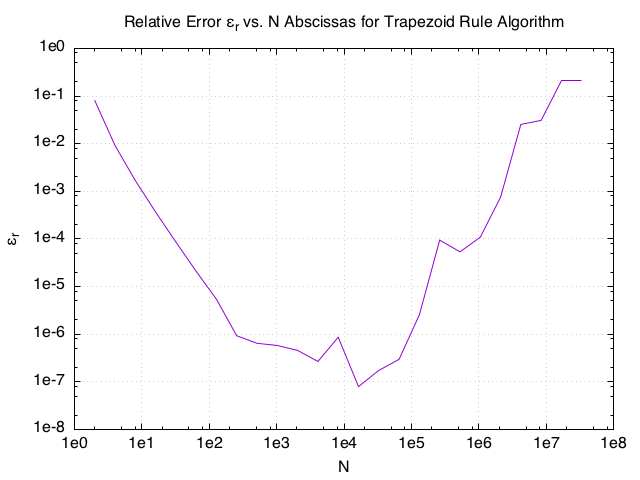
\includegraphics[scale=0.6]{trapezoid_rule.png}
	\caption{Relative error $\epsilon_r$ for the trapezoid rule algorithm as a function of the number of abscissa $N$.}
\end{figure}

In Figure 4, above, we see the relative error $\epsilon_r$ as a function of the number of abcissa $N$. For a trapezoid rule algorithm, we expect the optimal relative error $\epsilon_{opt}$ and optimal number of abcissa $N_{opt}$ to be given by the following:

\begin{equation}
	\epsilon_{opt} \sim \epsilon_{m}^{4/5}
\end{equation}
\begin{equation}
	N_{opt} \sim \epsilon_{m}^{-2/5}
\end{equation}

For single-precision measurements, (11) corresponds to $\sim 10^{-6}$, while (12) corresponds to $\sim 10^2$. Looking at Figure 4, we see the minimum relative error we obtain is $\sim 10^{-7}$, in fairly good agreement with our rough estimate. However, our optimal $N$ is $\sim 10^{4}$, in contrast with our estimate. It is worth noting, though, that for $N\sim 10^{2}$ we do reach a relative error of $\epsilon_{r}\sim 10^{-6}$. Finally, for a trapezoid rule algorithm, we expect the round-off error $\epsilon_{RO}$ and truncation error $\epsilon_{T}$ to scale in the following ways:
\begin{equation}
	\epsilon_{RO} \propto \sqrt{N}
\end{equation}
\begin{equation}
	\epsilon_{T} \propto N^{-2}
\end{equation}

For $N<N_{opt}$, which we take to be the computated value, rather than the theoretical value, we see that $\epsilon_{r}(N)$ follows a straight line in the log-log plot. It can be seen that the slope of this line is roughly $-2$ in the log-log plot, indicating $n\approx -2$, as expected. \\

For $N>N_{opt}$, we see that $\epsilon_{r}(N)$ seems to be following a parabolic path, which is not expected. Even if we approximate this path by a straight line it is clear the slope of this line in the log-log plot would be roughly $3$, in stark contrast to our expected value of $\frac{1}{2}$. The source of this discrepancy is likely due to some inefficiency in our algorithm's computation. An excessive number of computations may make the round-off error more severe than the best case scenario which the theoretical value estimates.

\begin{figure}[H]
	\centering
	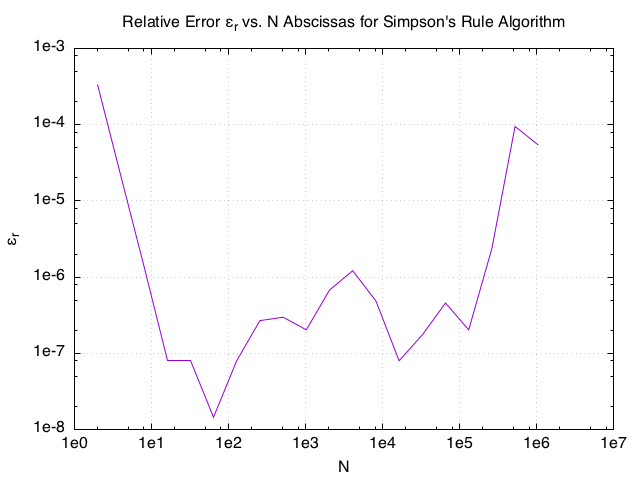
\includegraphics[scale=0.6]{simpsons_rule.png}
	\caption{Relative error $\epsilon_r$ for the Simpon's rule algorithm as a function of the number abscissa $N$.}
\end{figure}

In Figure 5, above, we see the relative error $\epsilon_r$ as a function of the number of abcissa $N$. For a Simpson's Rule algorithm, we expect the optimal relative error $\epsilon_{opt}$ and optimal number of abcissa $N_{opt}$ to be given by the following:
\begin{equation}
	\epsilon_{opt} \sim \epsilon_{m}^{8/9}
\end{equation}
\begin{equation}
	N_{opt} \sim \epsilon_{m}^{-2/9}
\end{equation}

For single-precision measurements, (15) corresponds to $\sim 10^{-7}$, while (16) corresponds to $\sim 10$. Looking at Figure 5, we see the minimum relative error we obtain is $\sim 10^{-7}$, in good agreement with our estimate. The optimal number of abcissa can be seen to be $\sim 10$, also in very good agreement with our estimate. Lastly, for a Simpson's Rule algorithm, we expect the round-off error $\epsilon_{RO}$ to follow (13), while the truncation error $\epsilon_{T}$ should scale in the following way:
\begin{equation}
	\epsilon_{T} \propto N^{-4}
\end{equation}

For $N<N_{opt}$, we see that $\epsilon_{r}(N)$ follows a straight line in the log-log plot. The slope of this line looks to be about $-4$ in the log-log plot, indicating $n\approx -4$, as expected.\\

For $N>N_{opt}$, but not too large, we see that $\epsilon_{r}(N)$, if approximated by a straight line, has a slope of roughly $-\frac{1}{2}$ in the log-log plot. This, of course, indicates $n\approx -\frac{1}{2}$, as we would expect. However, for large $N$, $\epsilon_{r}(N)$ follows a straight line in the log-log plot of slope roughly $2$, indicating $n\approx 2$. This is again in stark contrast with our estimate and is likely due to inefficiencies in our algorithm, which causes the round-off error to be more severe than estimated.

\begin{figure}[H]
	\centering
	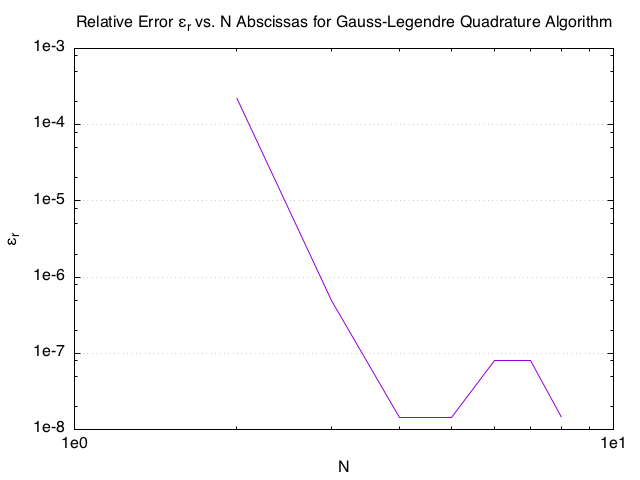
\includegraphics[scale=0.6]{GL_quad.png}
	\caption{Relative error $\epsilon_r$ for the Gauss-Legendre quadrature algorithm as a function of the number of abscissa $N$.}
\end{figure}

In Figure 6, we again see the relative error $\epsilon_r$ plotted as a function of the number of abcissa $N$. It is clear from the figure that we obtain $N_{opt}\sim 1$ and $\epsilon_{opt} \sim 10^{-8}$, making it by far the most efficient and precise algorithm. Note that as $N$ increases we begin to see the very start of the loss of precision to round-off error.

\subsection*{3.}

The code written to generate the random walk can be found in the source code \verb|prob3.cpp| in the appendix. Plots and data were generate by running \verb|prob3.sh|, also in the appendix. Figures 7-9, below, show $\sigma^{2}$, $s_3$, and $s_4$ for the random walk as a function of $n$.\\

For a random walker starting a position $x_0$ and taking unit length steps forward or backward, the position of the walker after $n$ steps is given by the recursion relation:
\begin{equation}
	\left.\begin{aligned}
		x_0 &= 0 \\
		x_n &= x_{n-1} + l_{n}
	\end{aligned}
	\right\}
\end{equation}
where $l_{n}$ is a random variable, equal to $\pm1$ with equal probability, giving the $n^{th}$ step. Plugging each $x_{k}$, $k=0,1, ...,n-1$, into (18) we obtain the closed form equation for $x_n$:
\begin{align}
	x_n &= x_0 + \sum\limits_{k=1}^{n} l_k \nonumber \\
		&= \sum\limits_{k=1}^{n} l_k
\end{align}
Finally, we note several facts about the $l_{k}$. Firstly, $l_{k}$ and $l_{j}$ are independent random variables for $k\neq j$. Secondly, the following expectation values can be derived easily from the definition:
\begin{subequations}
	\begin{align}
		\langle l_k \rangle &= 0 \\ 
		\langle l_k^2 \rangle &= 1 \\
		\langle l_k^3 \rangle &= 0 \\
		\langle l_k^4 \rangle &= 1
	\end{align}
\end{subequations}

\begin{figure}[H]
	\centering
	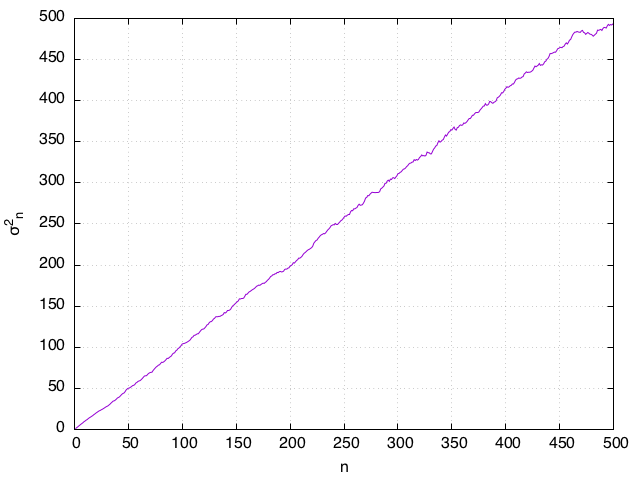
\includegraphics[scale=0.6]{sigma2.png}
	\caption{$\sigma^{2}$ as a function of the number of steps $n$ in the random walk.}
\end{figure}

Figure 7, above, shows the variance of $\sigma_{n}^2$ the final position after $n$ steps $x_n$ as a function of the number of steps $n$. Here, we calculate the variance using:
\begin{align}
	\sigma_n^2 &= \langle x_n^2 \rangle - \langle x_n \rangle^2 \nonumber \\
			   &= \langle x_n^2 \rangle
\end{align}
where we obtain the second line by comparing (19) and (20a). To obtain a theoretical estimate for the variance we expand $x_n^2$ using (19):
\begin{align}
	x_n^2 &= \left(\sum\limits_{k=1}^{n} l_k \right)^2 \nonumber \\
		  &= \sum\limits_{k=1}^{n} l_k^2 + 2\sum\limits_{k=1}^{n}\sum\limits_{j<k} l_k l_j \nonumber \\
	\implies \langle x_n^2 \rangle &= n
\end{align}
where we obtain the final line using the independence of the $l_k$, (20a), and (20b). Therefore, in the limit of large $n$ we expect:
\begin{equation}
	\sigma_n^2 = n
\end{equation}
Comparing this prediction to Figure 7, we see that our results are in very good agreement with (23). 

\begin{figure}[H]
	\centering
	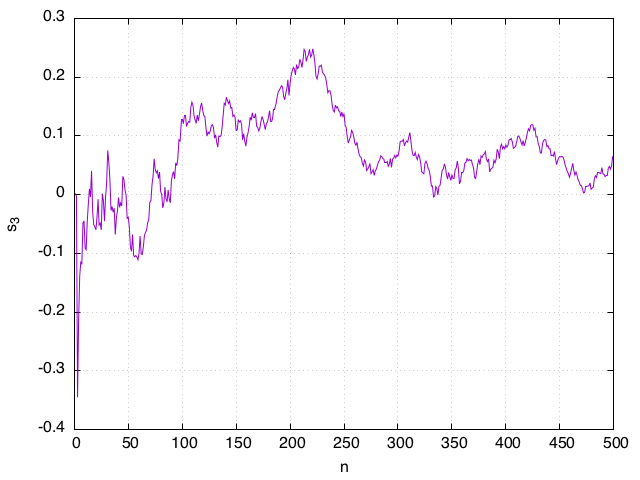
\includegraphics[scale=0.6]{s_3.png}
	\caption{$s_3$ as a function of the number of steps $n$ in the random walk.}
\end{figure}

Figure 8, above, shows $s_3$ as a function of $n$, where $s_3$ is given by:
\begin{equation}
	s_3 = \frac{\langle x_n^3 \rangle}{\sigma_n^3}
\end{equation}
To obtain a theoretical estimate for $s_3$ we expand $x_n^3$ using (19):
\begin{align}
	x_n^3 &= \left( \sum\limits_{k=1}^{n} l_{k} \right)^3 \nonumber \\
		  &= \sum\limits_{k=1}^{n} l_k^3 + 6\sum\limits_{k=1}^{n}\sum\limits_{j<k} l_k^2 l_j + 6\sum\limits_{k=1}^{n}\sum\limits_{j<k}\sum\limits_{i<j} l_k l_j l_i \nonumber \\
	\implies \langle x_n^3 \rangle &=0
\end{align}
where we obtain the final line using the independence of $l_k$, (20a), and (20c). Therefore, in the limit of large $n$ we expect:
\begin{equation}
	s_3 = 0
\end{equation}
Comparing this prediction to Figure 8, we see that our results are in fairly good agreement with (26).

\begin{figure}[H]
	\centering
	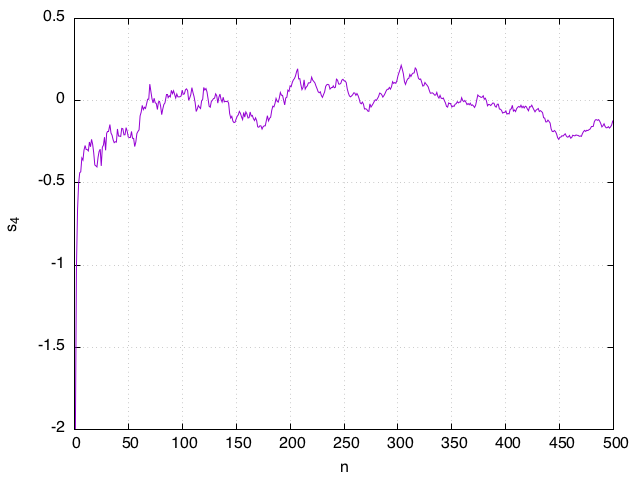
\includegraphics[scale=0.6]{s_4.png}
	\caption{$s_4$ as a function of the number of steps $n$ in the random walk.}
\end{figure}

Figure 9, above, shows $s_4$ as a function of $n$, where $s_4$is given by:
\begin{equation}
s_4 = \frac{\langle x_n^4\rangle}{\sigma_n^4} -3
\end{equation}

To obtain a theoretical estimate for $s_4$ we expand $x_n^4$ using (19):
\begin{align}
	x_n^4 =& \left( \sum\limits_{k=1}^{n} l_k \right) ^4 \nonumber \\
		  =& \sum\limits_{k=1}^{n} l_k^4 + 6\sum\limits_{k=1}^{n}\sum\limits_{j<k} l_k^2 l_j^2 + 4\sum\limits_{k=1}^{n}\sum\limits_{j<k} l_k^3 l_j \nonumber \\
		 & + 12\sum\limits_{k=1}^{n}\sum\limits_{j<k}\sum\limits_{i<j} l_k^2 l_j l_i + 24\sum\limits_{k=1}^{n}\sum\limits_{j<k}\sum\limits_{i<j}\sum\limits_{h<i} l_k l_j l_i l_h \nonumber \\
	\implies \langle x_n^4 \rangle =& n + 6\frac{n(n-1)}{2} \nonumber \\
								   =& 3n^2 -2n
\end{align}
where we obtain the final expression using the independence of the $l_k$ and (20). Therefore, in the limit of large $n$ we expect:
\begin{equation}
	s_4 = 0	
\end{equation}
where we have plugged in $\sigma^2_n=n$ and taken dropped terms approaching zero. Comparing this prediction to Figure 9, we see that our results are in very good agreement with (31). 

\clearpage

\begin{thebibliography}{1}

	\bibitem{projecteuclid}
	Lowan, Arnold N.; Davids, Norman; Levenson, Arthur.
	\emph{Table of the zeros of the Legendre polynomials of order 1-16 and the weight coefficients for Gauss' mechanical quadrature formula.}
	Bull. Amer. Math. Soc. 48 (1942), no. 10, 739--743.
	http://projecteuclid.org/euclid.bams/1183504772.

\end{thebibliography}


\clearpage

\subsection*{Appendix}

\subsubsection*{\texttt{prob1.cpp}:}

\inputminted[breaklines=true]{c}{prob1.cpp}

\subsubsection*{\texttt{prob1.sh}:}

\inputminted[breaklines=true]{sh}{prob1.sh}

\subsubsection*{\texttt{prob2.cpp}:}

\inputminted[breaklines=true]{c}{prob2.cpp}

\subsubsection*{\texttt{prob2.sh}:}

\inputminted[breaklines=true]{sh}{prob2.sh}

\subsubsection*{\texttt{prob3.cpp}:}

\inputminted[breaklines=true]{c}{prob3.cpp}

\subsubsection*{\texttt{prob3.sh}:}

\inputminted[breaklines=true]{sh}{prob3.sh}

\end{document}
